\documentclass[12pt,a4paper]{article}

\usepackage[utf8]{inputenc}
\usepackage[T1]{fontenc}
\usepackage[brazil]{babel}
\usepackage{indentfirst}

\usepackage[top=3cm,bottom=2cm,left=3cm,right=2cm]{geometry}
\usepackage{setspace}
\onehalfspacing
\usepackage{mathptmx}

\usepackage{graphicx}
\usepackage{booktabs}
\usepackage{multirow}
\usepackage{float}
\usepackage{caption}
\usepackage{amsmath,amssymb}
\usepackage{listings}
\usepackage{xcolor}
\usepackage[hidelinks]{hyperref}
\usepackage{xurl}

\captionsetup{font=small,labelsep=endash,justification=centering}
\captionsetup[table]{position=top}
\captionsetup[figure]{position=top}

\newcommand{\fonte}[1]{
	\vspace{-2mm}
	\begin{center}\footnotesize Fonte: #1\end{center}
}
\newcommand{\fontedados}{elaborada pelos autores com dados da SSPDS/CE e do IBGE.}

\lstdefinestyle{python}{
	language=Python,
	basicstyle=\ttfamily\scriptsize,
	keywordstyle=\color{blue},
	commentstyle=\color{gray},
	stringstyle=\color{teal},
	numbers=left, numberstyle=\tiny, numbersep=8pt,
	breaklines=true, frame=single, showstringspaces=false,
	extendedchars=true,
	literate=
	{á}{{\'a}}1 {é}{{\'e}}1 {í}{{\'i}}1 {ó}{{\'o}}1 {ú}{{\'u}}1
	{Á}{{\'A}}1 {É}{{\'E}}1 {Í}{{\'I}}1 {Ó}{{\'O}}1 {Ú}{{\'U}}1
	{à}{{\`a}}1 {ã}{{\~a}}1 {õ}{{\~o}}1 {Ã}{{\~A}}1 {Õ}{{\~O}}1
	{ç}{{\c c}}1 {Ç}{{\c C}}1 {ê}{{\^e}}1 {â}{{\^a}}1 {ô}{{\^o}}1
	{ª}{{\textsuperscript{a}}}1 {×}{{$\times$}}1
}

\begin{document}
	
	\begin{titlepage}
		\begin{center}
			
			
\includegraphics[width=0.65\textwidth]{figuras/logo-unifor.png}\\[0.5cm]
			
			{\large CENTRO DE CIÊNCIAS TECNOLÓGICAS -- CCT}\\[0.3cm]
			{\large Métodos Quantitativos em Computação}\\[0.2cm]
			{\normalsize Professor Cledinaldo Castro Araújo}
			
			\vfill
			
			{\Huge \textbf{Análise de Regressão Linear}}\\[0.6cm]
			{\Large Crimes Violentos Letais Intencionais (CVLI), população e\\ PIB per capita nos municípios do Ceará}
			
			\vfill
			
			{\large \textbf{Alunos:}}\\[0.2cm]
			{\large Guilherme Azevedo --- Matrícula: 2510423}\\[0.1cm]
			{\large Matheus Cruz --- Matrícula: 2517389}\\[0.1cm]
			{\large Samuel Lopes --- Matrícula: 2510371}\\[0.1cm]
			{\large Enzo Fernandes --- Matrícula: 2510425}\\[0.1cm]
			{\large Rodrigo Temporal --- Matrícula: 2510402}
			
			\vfill
			
			{\large Fortaleza, Outubro de 2026}
			
		\end{center}
	\end{titlepage}
	
	\renewcommand{\contentsname}{Sumário}
	\tableofcontents
	\newpage
	
	\section{Introdução}
	
	Os Crimes Violentos Letais Intencionais (CVLI) --- homicídio doloso, feminicídio, lesão corporal seguida de morte e latrocínio --- são o principal indicador de violência letal acompanhado pela Secretaria da Segurança Pública e Defesa Social do Ceará (SSPDS/CE). A análise descritiva realizada no trabalho anterior da disciplina mostrou que esses crimes se concentram fortemente em poucos municípios: Fortaleza, sozinha, respondeu por cerca de 36\% dos 59.340 registros de 2009 a 2025.
	
	Esse retrato agregado, porém, esconde mudanças no nível municipal. O Ceará fechou 2022 e 2023 com exatamente o mesmo número de homicídios (2.970), mas o Comitê de Prevenção e Combate à Violência da Assembleia Legislativa mostrou que, de um ano para o outro, 80 municípios tiveram aumento e 75 tiveram redução, e que 11 dos 19 municípios da Região Metropolitana de Fortaleza (RMF) registraram alta. O comitê classificou o fenômeno como uma interiorização da violência armada e defendeu ações de prevenção planejadas por região (O POVO, 2024a). Na avaliação da própria SSPDS/CE, a principal força por trás dos homicídios no estado é a disputa territorial entre facções criminosas, que em 2025 levou a mais prisões de faccionados na RMF do que na capital (DIÁRIO DO NORDESTE, 2026).
	
	Essa concentração levanta uma pergunta que a estatística descritiva, sozinha, não responde: o número de CVLI de um município é explicado apenas pelo seu tamanho populacional, ou o nível de atividade econômica também se associa à violência letal? Responder a essa pergunta exige um modelo que avalie o efeito de cada variável mantendo as demais constantes, o que é o propósito da análise de regressão linear.
	
	Este trabalho estima e valida modelos de regressão linear simples e múltipla para os 184 municípios do Ceará. A variável dependente é o total de CVLI no triênio 2021--2023, e as variáveis explicativas são a população residente do Censo Demográfico 2022 e o PIB per capita municipal de 2022, ambos do IBGE. O estudo percorre as etapas de identificação das variáveis, diagramas de dispersão, coeficientes de correlação, estimação dos modelos, qualidade do ajuste, análise de variância, diagnóstico dos resíduos e previsões.
	
	\newpage
	
	\section{Objetivos}
	
	\subsection{Objetivo Geral}
	
	Estimar e validar um modelo de regressão linear que explique o número de Crimes Violentos Letais Intencionais dos municípios do Ceará no período de 2021 a 2023 a partir da população residente e do PIB per capita municipal.
	
	\subsection{Objetivos Específicos}
	
	\begin{itemize}
		\item Identificar e caracterizar as variáveis dependente e explicativas no nível municipal;
		\item Avaliar, por meio de diagramas de dispersão e coeficientes de correlação, a relação entre o número de CVLI, a população e o PIB per capita;
		\item Estimar os modelos de regressão linear simples (população) e múltipla (população e PIB per capita) e interpretar seus coeficientes;
		\item Avaliar a qualidade do ajuste pelo coeficiente de determinação, pela análise de variância e pelo diagnóstico dos resíduos;
		\item Comparar a especificação na escala original com a especificação em logaritmos, justificando a escolha do modelo final;
		\item Realizar previsões com intervalos de confiança e de previsão para um município de perfil definido.
	\end{itemize}
	
	\newpage
	
	\section{Metodologia}
	
	\subsection{Natureza do estudo e unidade de análise}
	
	Trata-se de um estudo quantitativo, de natureza correlacional, com dados secundários de repositórios públicos. A unidade de análise é o município: os 184 municípios do Ceará compõem a base completa (não há amostragem).
	
	\subsection{Bancos de dados e fontes}
	
	\begin{itemize}
		\item \textbf{CVLI:} base de indicadores detalhados de 2009 a 2025 da SSPDS/CE, com um registro por vítima (59.340 registros). Foram contados os CVLI de cada município nos anos de 2021, 2022 e 2023.
		\item \textbf{População:} Censo Demográfico 2022 do IBGE, tabela 4714 do SIDRA (população residente).
		\item \textbf{PIB per capita:} base de dados do PIB dos Municípios do IBGE (2010--2023), ano de referência 2022.
	\end{itemize}
	
	O triênio 2021--2023 foi escolhido por estar centrado no ano do Censo e do PIB utilizados, e por reduzir a variação aleatória de municípios pequenos, que registram poucos casos em um único ano. Essa variação é grande: São João do Jaguaribe, com menos de 6 mil habitantes, registrou 23 homicídios em 2021, o maior número de sua série histórica, e apenas dois até julho de 2022 (O POVO, 2022b). Somar três anos evita que um pico isolado de um único ano defina a posição do município no modelo. O total obtido, 9.239 CVLI, coincide com a soma da série anual oficial da SSPDS/CE para os três anos (3.299, 2.970 e 2.970).
	
	\subsection{Tratamento dos dados}
	
	\begin{enumerate}
		\item Os arquivos brutos do IBGE foram mantidos sem edição. O script \texttt{preparar\_ibge.py} extrai a população dos 184 municípios, filtra o PIB per capita do Ceará em 2022 e une as duas bases (Anexo A).
		\item O script \texttt{analise\_regressao.py} agrega os CVLI por município e une essa contagem à base do IBGE (Anexo B). Como os nomes dos municípios diferem entre as fontes (acentos e caixa), a junção usa os nomes normalizados; os 184 municípios casaram nas duas etapas.
		\item Três municípios não registraram CVLI no período (Antonina do Norte, Baixio e Granjeiro). Para permitir o uso de logaritmos, a variável dependente foi transformada em $\ln(\text{CVLI}+1)$.
		\item As variáveis explicativas foram transformadas em $\ln(\text{população})$ e $\ln(\text{PIB per capita})$. A escolha da escala logarítmica é justificada na Seção~\ref{sec:escala}.
	\end{enumerate}
	
	\subsection{Métodos e ferramentas}
	
	Os modelos foram estimados por Mínimos Quadrados Ordinários (MQO). A análise inclui correlações de Pearson e Spearman, testes $t$ dos coeficientes, coeficiente de determinação, análise de variância (ANOVA) com teste $F$ global e teste $F$ entre modelos aninhados, fator de inflação da variância (VIF), teste de Shapiro-Wilk para a normalidade dos resíduos, teste de Breusch-Pagan para a homocedasticidade, distância de Cook para pontos influentes e previsões com intervalos de 95\%. Adotou-se nível de significância de 5\%.
	
	A análise foi feita em \textbf{Python 3.15}, com as bibliotecas \texttt{pandas} (tratamento e junção das bases), \texttt{numpy} (transformações), \texttt{statsmodels} (modelos, ANOVA e diagnósticos; SEABOLD; PERKTOLD, 2010), \texttt{SciPy} (correlações e Shapiro-Wilk) e \texttt{matplotlib} (gráficos). As funções de leitura, conversão e junção dos dados são verificadas por testes automatizados com \texttt{pytest}. O código completo está nos Anexos e no repositório do projeto.
	
	\newpage
	
	\section{Justificativa}
	
	Contagens absolutas de crimes tendem a acompanhar o tamanho da população: municípios maiores têm mais pessoas expostas e, por isso, mais ocorrências. Comparar municípios apenas pelo número de casos confunde esse efeito de escala com características locais que podem estar associadas à violência. A regressão múltipla permite separar esses efeitos e responder se, para municípios de mesmo porte, o nível econômico se associa a mais ou menos CVLI.
	
	Do ponto de vista da gestão pública, essa informação ajuda a definir quais municípios apresentam mais casos do que o esperado para o seu perfil, o que pode orientar a alocação de efetivo policial e de programas de prevenção. É o tipo de evidência que o comitê da Assembleia Legislativa considerou necessária ao recomendar ações regionalizadas, depois de constatar que a estabilidade do total estadual escondia altas em dezenas de municípios (O POVO, 2024a). Do ponto de vista metodológico, o estudo mostra por que um coeficiente de determinação alto não basta para validar um modelo: como se verá na Seção~\ref{sec:escala}, o modelo na escala original atinge $R^2$ de 0,97, mas é dominado por um único município e viola a hipótese de normalidade dos resíduos.
	
	\newpage
	
	\section{Referencial Teórico}
	
	\subsection{Correlação}
	
	O coeficiente de correlação de Pearson mede a intensidade da relação \emph{linear} entre duas variáveis quantitativas e varia de $-1$ a $1$:
	\[
	r = \frac{\sum (x_i-\bar{x})(y_i-\bar{y})}{\sqrt{\sum (x_i-\bar{x})^2\,\sum (y_i-\bar{y})^2}}.
	\]
	O coeficiente de Spearman ($\rho$) aplica a mesma fórmula aos postos das observações, medindo associação monótona e sendo menos sensível a valores extremos (BUSSAB; MORETTIN, 2017).
	
	\subsection{Modelo de regressão linear}
	
	O modelo de regressão linear múltipla com $k$ variáveis explicativas é
	\[
	Y_i = \beta_0 + \beta_1 X_{1i} + \dots + \beta_k X_{ki} + \varepsilon_i,
	\]
	em que os coeficientes são estimados por MQO, minimizando a soma dos quadrados dos resíduos $\sum e_i^2$. A inferência sobre os coeficientes (testes $t$ e intervalos de confiança) supõe que os erros sejam independentes, com média zero, variância constante (homocedasticidade) e distribuição normal, e que as variáveis explicativas não sejam fortemente colineares (MONTGOMERY; PECK; VINING, 2012).
	
	\subsection{Modelo log-log}
	
	Quando $Y$ e $X$ são transformados em logaritmos, o coeficiente $\beta_j$ é interpretado como uma \emph{elasticidade}: um aumento de 1\% em $X_j$ associa-se a uma variação de aproximadamente $\beta_j$\% em $Y$, mantidas as demais variáveis constantes. A transformação reduz a assimetria de variáveis com grande amplitude e diminui a influência de valores extremos (GUJARATI; PORTER, 2011). Como há municípios com zero casos, usa-se $\ln(Y+1)$, que coincide aproximadamente com $\ln Y$ para contagens maiores.
	
	\subsection{Qualidade do ajuste e análise de variância}
	
	A variabilidade total da variável dependente se decompõe em $SQT = SQReg + SQRes$. O coeficiente de determinação $R^2 = 1 - SQRes/SQT$ indica a proporção da variabilidade explicada pelo modelo, e o $R^2$ ajustado,
	\[
	R^2_{aj} = 1 - (1-R^2)\frac{n-1}{n-k-1},
	\]
	penaliza a inclusão de variáveis que pouco contribuem. A ANOVA testa a hipótese de que todos os coeficientes angulares são nulos pela estatística
	\[
	F = \frac{SQReg/k}{SQRes/(n-k-1)},
	\]
	e o teste $F$ entre modelos aninhados verifica se a inclusão de uma nova variável reduz significativamente a soma dos quadrados dos resíduos.
	
	\subsection{Diagnóstico do modelo}
	
	\begin{itemize}
		\item \textbf{Normalidade dos resíduos:} teste de Shapiro-Wilk, cuja hipótese nula é a de que os resíduos seguem distribuição normal (SHAPIRO; WILK, 1965), complementado pelo gráfico quantil-quantil (Q-Q).
		\item \textbf{Homocedasticidade:} teste de Breusch-Pagan, cuja hipótese nula é a de variância constante dos erros (BREUSCH; PAGAN, 1979), complementado pelo gráfico de resíduos contra valores ajustados.
		\item \textbf{Multicolinearidade:} fator de inflação da variância, $VIF_j = 1/(1-R_j^2)$, em que $R_j^2$ vem da regressão de $X_j$ sobre as demais explicativas. Valores abaixo de 5 costumam ser considerados aceitáveis.
		\item \textbf{Pontos influentes:} distância de Cook, que mede o quanto os coeficientes mudam quando uma observação é retirada. Valores acima de 1 indicam observações que dominam o ajuste (COOK, 1977).
	\end{itemize}
	
	\subsection{Previsão}
	
	Para um novo conjunto de valores das variáveis explicativas, o intervalo de confiança estima onde está o valor \emph{médio} de $Y$ para municípios com esse perfil, enquanto o intervalo de previsão estima onde deve cair o valor de \emph{um} município específico. O intervalo de previsão é sempre mais largo, pois incorpora também a variabilidade dos erros individuais.
	
	\newpage
	
	\section{Desenvolvimento}
	
	\subsection{Identificação das variáveis}
	
	\begin{table}[H]
		\centering
		\caption{Variáveis do estudo}
		\label{tab:variaveis}
		\small
		\resizebox{\textwidth}{!}{%
			\begin{tabular}{llll}
				\toprule
				\textbf{Variável} & \textbf{Papel no modelo} & \textbf{Tipo} & \textbf{Fonte} \\
				\midrule
				CVLI 2021--2023 ($Y$)          & dependente  & quantitativa discreta (contagem) & SSPDS/CE \\
				População residente ($X_1$)    & explicativa & quantitativa discreta             & IBGE, Censo 2022 \\
				PIB per capita ($X_2$)         & explicativa & quantitativa contínua (R\$)       & IBGE, PIB dos Municípios 2022 \\
				\bottomrule
		\end{tabular}}
	\end{table}
	\fonte{elaborada pelos autores.}
	
	\begin{table}[H]
		\centering
		\caption{Amplitude das variáveis nos 184 municípios do Ceará}
		\label{tab:amplitude}
		\small
		\resizebox{\textwidth}{!}{%
			\begin{tabular}{lrlrl}
				\toprule
				\textbf{Variável} & \textbf{Mínimo} & \textbf{Município} & \textbf{Máximo} & \textbf{Município} \\
				\midrule
				CVLI 2021--2023              & 0        & Antonina do Norte, Baixio e Granjeiro & 2.488     & Fortaleza \\
				População (hab.)             & 4.841    & Granjeiro                              & 2.428.708 & Fortaleza \\
				PIB per capita (R\$)         & 8.598,70 & Pires Ferreira                         & 127.619,92 & São Gonçalo do Amarante \\
				\bottomrule
		\end{tabular}}
	\end{table}
	\fonte{\fontedados}
	
	Entende-se, pelas Tabelas~\ref{tab:variaveis} e~\ref{tab:amplitude}, que as três variáveis são quantitativas e apresentam amplitude muito grande. A população de Fortaleza é cerca de 500 vezes a de Granjeiro, e o PIB per capita de São Gonçalo do Amarante, município do Complexo Industrial e Portuário do Pecém, é quase 15 vezes o de Pires Ferreira. Variáveis com esse grau de assimetria tendem a produzir regressões dominadas pelos poucos valores extremos, o que motiva a análise em escala logarítmica.
	
	A assimetria reflete a geografia do estado. Fortaleza concentra 27,61\% da população cearense (IPECE, 2023), e a Região Metropolitana reúne cerca de 44\% (BANCO DO NORDESTE, 2023). Entre os Censos de 2010 e 2022, a capital perdeu cerca de 23,5 mil moradores, enquanto 71 dos 184 municípios perderam população (DIÁRIO DO NORDESTE, 2023a) e municípios vizinhos cresceram rapidamente, como o Eusébio, com aumento de 80\% (DIÁRIO DO NORDESTE, 2023b). No PIB per capita, a concentração é ainda maior: em 2020, 89,7\% dos municípios tinham PIB per capita abaixo da média estadual, e São Gonçalo do Amarante lidera o ranking desde 2017 por causa do Complexo Industrial e Portuário do Pecém (ECONOMIC NEWS BRASIL, 2022). O segundo colocado, o Eusébio, deve sua posição em grande parte à sede de uma grande indústria de alimentos (O POVO, 2023b).
	
	\subsection{Diagramas de dispersão}
	
	\begin{figure}[H]
		\centering
		\caption{Diagrama de dispersão entre $\ln(\text{CVLI}+1)$ e $\ln(\text{população})$, municípios do Ceará}
		\label{fig:disp-pop}
		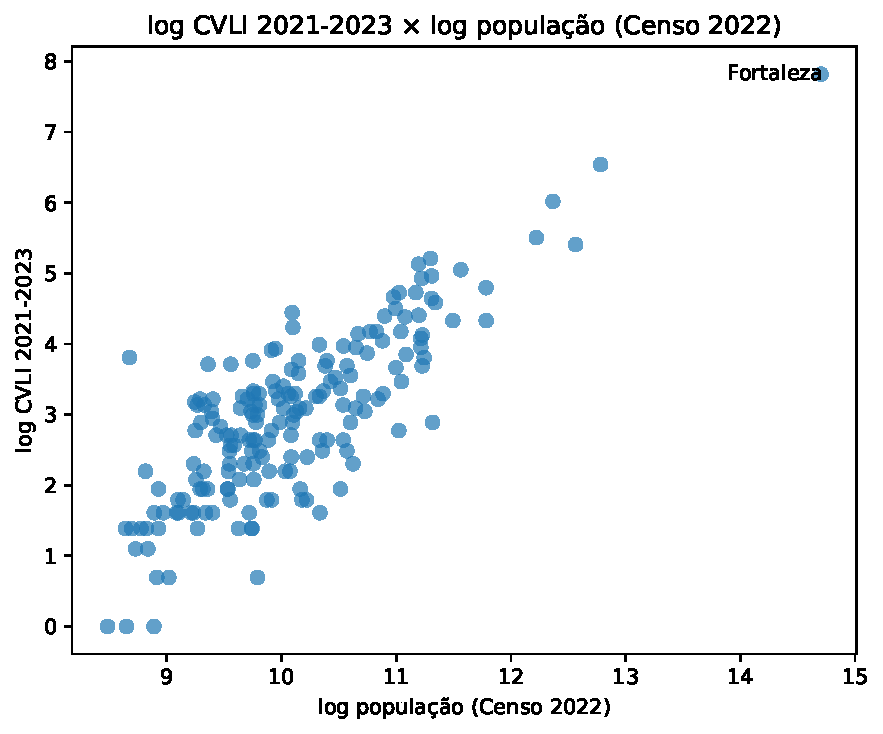
\includegraphics[width=0.68\textwidth]{figuras/dispersao_populacao.pdf}
	\end{figure}
	\fonte{\fontedados}
	
	Observa-se, na Figura~\ref{fig:disp-pop}, uma relação positiva, aproximadamente linear e intensa: quanto maior a população do município, maior o número de CVLI, e a nuvem de pontos se distribui em torno de uma reta ao longo de toda a faixa de tamanhos. Fortaleza, no extremo superior direito, segue a mesma tendência dos demais municípios, sem se destacar como ponto atípico nessa escala. A dispersão vertical é maior entre os municípios pequenos, nos quais poucos casos a mais ou a menos produzem variações relativas grandes.
	
	\begin{figure}[H]
		\centering
		\caption{Diagrama de dispersão entre $\ln(\text{CVLI}+1)$ e $\ln(\text{PIB per capita})$, municípios do Ceará}
		\label{fig:disp-pib}
		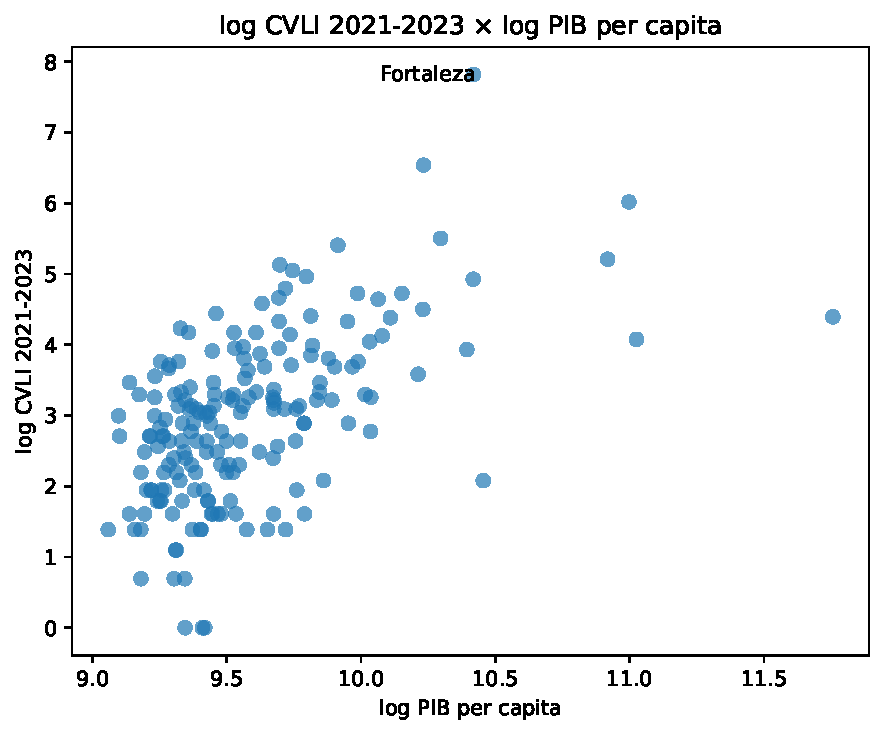
\includegraphics[width=0.68\textwidth]{figuras/dispersao_pib.pdf}
	\end{figure}
	\fonte{\fontedados}
	
	Conclui-se, pela Figura~\ref{fig:disp-pib}, que a relação entre CVLI e PIB per capita também é positiva, porém mais fraca e mais dispersa do que a relação com a população. A maioria dos municípios concentra-se em uma faixa estreita de PIB per capita, e alguns poucos pontos à direita --- municípios com atividade industrial ou portuária, como São Gonçalo do Amarante --- se afastam do padrão, com PIB per capita elevado e número de casos intermediário. Esses pontos mostram que o PIB per capita mede a produção do município dividida pela população, e não a renda de quem mora nele: Eusébio e Maracanaú, por exemplo, estão entre os dez maiores PIBs per capita do estado justamente por serem grandes polos de produção (IPECE, 2025).
	
	\subsection{Coeficientes de correlação}
	
	\begin{table}[H]
		\centering
		\caption{Coeficientes de correlação entre as variáveis em escala logarítmica}
		\label{tab:correlacao}
		\begin{tabular}{lcccc}
			\toprule
			\textbf{Par de variáveis} & \textbf{Pearson ($r$)} & \textbf{$p$-valor} & \textbf{Spearman ($\rho$)} & \textbf{$p$-valor} \\
			\midrule
			$\ln(\text{CVLI}+1)$ e $\ln(\text{população})$       & 0,815 & $<0{,}001$ & 0,743 & $<0{,}001$ \\
			$\ln(\text{CVLI}+1)$ e $\ln(\text{PIB per capita})$  & 0,560 & $<0{,}001$ & 0,539 & $<0{,}001$ \\
			$\ln(\text{população})$ e $\ln(\text{PIB per capita})$ & 0,512 & $<0{,}001$ & 0,463 & $<0{,}001$ \\
			\bottomrule
		\end{tabular}
	\end{table}
	\fonte{\fontedados}
	
	Entende-se, pela Tabela~\ref{tab:correlacao}, que a população tem correlação forte com o número de CVLI ($r = 0{,}815$) e o PIB per capita, correlação moderada ($r = 0{,}560$), ambas positivas e significativas. Os coeficientes de Spearman, próximos aos de Pearson, confirmam que as associações não dependem de poucos valores extremos. A correlação moderada entre as duas explicativas ($r = 0{,}512$) indica que municípios mais populosos também tendem a ter PIB per capita maior, o que exige verificar, no modelo múltiplo, se há multicolinearidade e se o PIB per capita acrescenta explicação além da população.
	
	\subsection{Estimação dos modelos}
	
	\begin{table}[H]
		\centering
		\caption{Modelo de regressão linear simples: $\ln(\text{CVLI}+1)$ em função de $\ln(\text{população})$}
		\label{tab:simples}
		\begin{tabular}{lccccc}
			\toprule
			\textbf{Termo} & \textbf{Coeficiente} & \textbf{Erro padrão} & \textbf{$t$} & \textbf{$p$-valor} & \textbf{IC 95\%} \\
			\midrule
			Intercepto              & $-8{,}138$ & 0,587 & $-13{,}86$ & $<0{,}001$ & $[-9{,}296;\ -6{,}979]$ \\
			$\ln(\text{população})$ & $1{,}101$  & 0,058 & $18{,}99$  & $<0{,}001$ & $[0{,}987;\ 1{,}215]$ \\
			\bottomrule
		\end{tabular}
	\end{table}
	\fonte{\fontedados}
	
	Conclui-se, pela Tabela~\ref{tab:simples}, que o modelo simples é
	\[
	\widehat{\ln(\text{CVLI}+1)} = -8{,}138 + 1{,}101\,\ln(\text{população}),
	\]
	com coeficiente angular significativo. A elasticidade estimada de 1,10, cujo intervalo de confiança fica inteiramente acima de 1, indica que o número de CVLI cresce um pouco \emph{mais} do que proporcionalmente à população: um município 1\% maior tem, em média, cerca de 1,1\% mais casos.
	
	\begin{table}[H]
		\centering
		\caption{Modelo de regressão linear múltipla: $\ln(\text{CVLI}+1)$ em função de $\ln(\text{população})$ e $\ln(\text{PIB per capita})$}
		\label{tab:multiplo}
		\small
		\resizebox{\textwidth}{!}{%
			\begin{tabular}{lcccccc}
				\toprule
				\textbf{Termo} & \textbf{Coeficiente} & \textbf{Erro padrão} & \textbf{$t$} & \textbf{$p$-valor} & \textbf{IC 95\%} & \textbf{VIF} \\
				\midrule
				Intercepto                   & $-12{,}591$ & 1,242 & $-10{,}14$ & $<0{,}001$ & $[-15{,}041;\ -10{,}140]$ & --- \\
				$\ln(\text{população})$      & $0{,}967$   & 0,065 & $14{,}92$  & $<0{,}001$ & $[0{,}839;\ 1{,}095]$ & 1,355 \\
				$\ln(\text{PIB per capita})$ & $0{,}605$   & 0,150 & $4{,}03$   & $<0{,}001$ & $[0{,}309;\ 0{,}902]$ & 1,355 \\
				\bottomrule
		\end{tabular}}
	\end{table}
	\fonte{\fontedados}
	
	Entende-se, pela Tabela~\ref{tab:multiplo}, que o modelo múltiplo estimado é
	\[
	\widehat{\ln(\text{CVLI}+1)} = -12{,}591 + 0{,}967\,\ln(\text{população}) + 0{,}605\,\ln(\text{PIB per capita}),
	\]
	com os dois coeficientes significativos. Mantido o PIB per capita constante, um aumento de 1\% na população associa-se a cerca de 0,97\% mais CVLI; como o intervalo de confiança dessa elasticidade contém 1, não se rejeita que, para municípios de mesmo nível econômico, os casos cresçam na mesma proporção da população. Parte do efeito ``mais que proporcional'' do modelo simples, portanto, estava associada ao PIB per capita.
	
	Esse resultado é coerente com a desconcentração da violência letal observada na própria base da SSPDS/CE. A participação de Fortaleza no total de CVLI caiu de 41,8\% em 2009--2017 para 31,3\% em 2018--2020 e 26,9\% em 2021--2023 --- praticamente a mesma fatia que a capital tem da população do estado (27,61\%). Em outras palavras, no período analisado a capital já não tem mais casos do que seu tamanho prevê; a violência se espalhou pela Região Metropolitana e pelo interior, como no caso de Itapipoca, que em 2023 viu os homicídios dispararem por causa de um conflito entre facções depois de ter sido apontada como um dos municípios menos violentos do Nordeste (O POVO, 2023a).
	
	Mantida a população constante, um PIB per capita 1\% maior associa-se a cerca de 0,61\% mais CVLI. Essa relação positiva não deve ser lida como causal: no Ceará, os maiores PIBs per capita estão em municípios industrializados e integrados à Região Metropolitana de Fortaleza (como Maracanaú, Eusébio, Aquiraz e São Gonçalo do Amarante), de modo que o PIB per capita funciona, no modelo, como um indicador de urbanização e dinamismo econômico --- contextos que, como discutido no trabalho anterior, concentraram as disputas entre facções criminosas no estado. Em maio de 2022, por exemplo, quase 60\% dos assassinatos do Ceará ocorreram em Fortaleza e na RMF, e pesquisador do Laboratório de Estudos da Violência da UFC associou a alta a tensões entre facções rivais em Maracanaú (O POVO, 2022a). Os VIF de 1,355, bem abaixo de 5, indicam que a correlação entre as explicativas não compromete as estimativas.
	
	\subsection{Coeficiente de determinação e qualidade do ajuste}
	
	\begin{table}[H]
		\centering
		\caption{Qualidade do ajuste dos modelos simples e múltiplo (escala logarítmica)}
		\label{tab:ajuste}
		\begin{tabular}{lcc}
			\toprule
			\textbf{Medida} & \textbf{Simples} & \textbf{Múltiplo} \\
			\midrule
			$R^2$                        & 0,665 & 0,692 \\
			$R^2$ ajustado               & 0,663 & 0,689 \\
			Erro padrão dos resíduos     & 0,694 & 0,667 \\
			Estatística $F$              & 360,80 & 203,57 \\
			$p$-valor do teste $F$       & $<0{,}001$ & $<0{,}001$ \\
			Observações                  & 184 & 184 \\
			\bottomrule
		\end{tabular}
	\end{table}
	\fonte{\fontedados}
	
	Observa-se, na Tabela~\ref{tab:ajuste}, que a população, sozinha, explica 66,5\% da variabilidade de $\ln(\text{CVLI}+1)$ entre os municípios, e que a inclusão do PIB per capita eleva o coeficiente de determinação para 69,2\%. O aumento também aparece no $R^2$ ajustado (de 0,663 para 0,689) e na redução do erro padrão dos resíduos, o que indica que o ganho não é apenas efeito de acrescentar uma variável ao modelo. Cerca de 31\% da variabilidade permanece sem explicação, atribuível a fatores não incluídos, como a dinâmica local de facções criminosas e características demográficas e sociais de cada município.
	
	\subsubsection{Escala original versus escala logarítmica}
	\label{sec:escala}
	
	\begin{table}[H]
		\centering
		\caption{Comparação do modelo múltiplo na escala original e na escala logarítmica}
		\label{tab:escala}
		\begin{tabular}{lcc}
			\toprule
			\textbf{Medida} & \textbf{Escala original} & \textbf{Escala logarítmica} \\
			\midrule
			$R^2$                                   & 0,970 & 0,692 \\
			Shapiro-Wilk ($W$; $p$-valor)           & 0,644; $<0{,}001$ & 0,996; 0,916 \\
			Breusch-Pagan ($p$-valor)               & 0,006 & 0,036 \\
			Maior distância de Cook (município)     & 182,95 (Fortaleza) & 0,128 (São João do Jaguaribe) \\
			\bottomrule
		\end{tabular}
	\end{table}
	\fonte{\fontedados{} Escala original obtida executando \texttt{analise\_regressao.py} com \texttt{USAR\_LOG = False}.}
	
	Conclui-se, pela Tabela~\ref{tab:escala}, que o $R^2$ de 0,970 do modelo na escala original é enganoso. A distância de Cook de Fortaleza, 182,95, mostra que esse único município determina praticamente sozinho a reta estimada: com 2,4 milhões de habitantes e 2.488 casos, ele cria uma correlação quase perfeita que não representa os outros 183 municípios. Além disso, os resíduos desse modelo rejeitam fortemente a normalidade e apresentam heterocedasticidade marcante. Na escala logarítmica, o $R^2$ é menor, mas os resíduos são compatíveis com a normalidade e nenhuma observação domina o ajuste, o que torna válidas as inferências. Por isso, o modelo logarítmico foi adotado como modelo final.
	
	\subsection{Análise de variância e validação do modelo}
	
	\begin{table}[H]
		\centering
		\caption{Análise de variância (ANOVA) do modelo de regressão múltipla}
		\label{tab:anova}
		\begin{tabular}{lccccc}
			\toprule
			\textbf{Fonte de variação} & \textbf{SQ} & \textbf{gl} & \textbf{QM} & \textbf{$F$} & \textbf{$p$-valor} \\
			\midrule
			Regressão & 180,881 & 2   & 90,440 & 203,57 & $<0{,}001$ \\
			Resíduos  & 80,413  & 181 & 0,444  &        &  \\
			Total     & 261,294 & 183 &        &        &  \\
			\bottomrule
		\end{tabular}
	\end{table}
	\fonte{\fontedados}
	
	Entende-se, pela Tabela~\ref{tab:anova}, que a regressão explica 180,881 das 261,294 unidades de variabilidade total ($R^2 = 0{,}692$) e que a estatística $F = 203{,}57$ leva à rejeição da hipótese de que os dois coeficientes angulares sejam nulos ($p < 0{,}001$). O modelo, portanto, é globalmente significativo.
	
	Para verificar se o PIB per capita deve permanecer no modelo, aplicou-se o teste $F$ entre o modelo simples e o múltiplo. A inclusão do PIB per capita reduziu a soma dos quadrados dos resíduos de 87,612 para 80,413, com $F = 16{,}20$ ($p = 0{,}0001$). Esse valor coincide com o quadrado da estatística $t$ do coeficiente ($4{,}03^2 \approx 16{,}2$), como esperado quando se acrescenta uma única variável, e confirma que o modelo múltiplo é superior ao simples.
	
	\subsection{Análise dos resíduos}
	
	\begin{figure}[H]
		\centering
		\caption{Diagnóstico gráfico dos resíduos do modelo de regressão múltipla}
		\label{fig:residuos}
		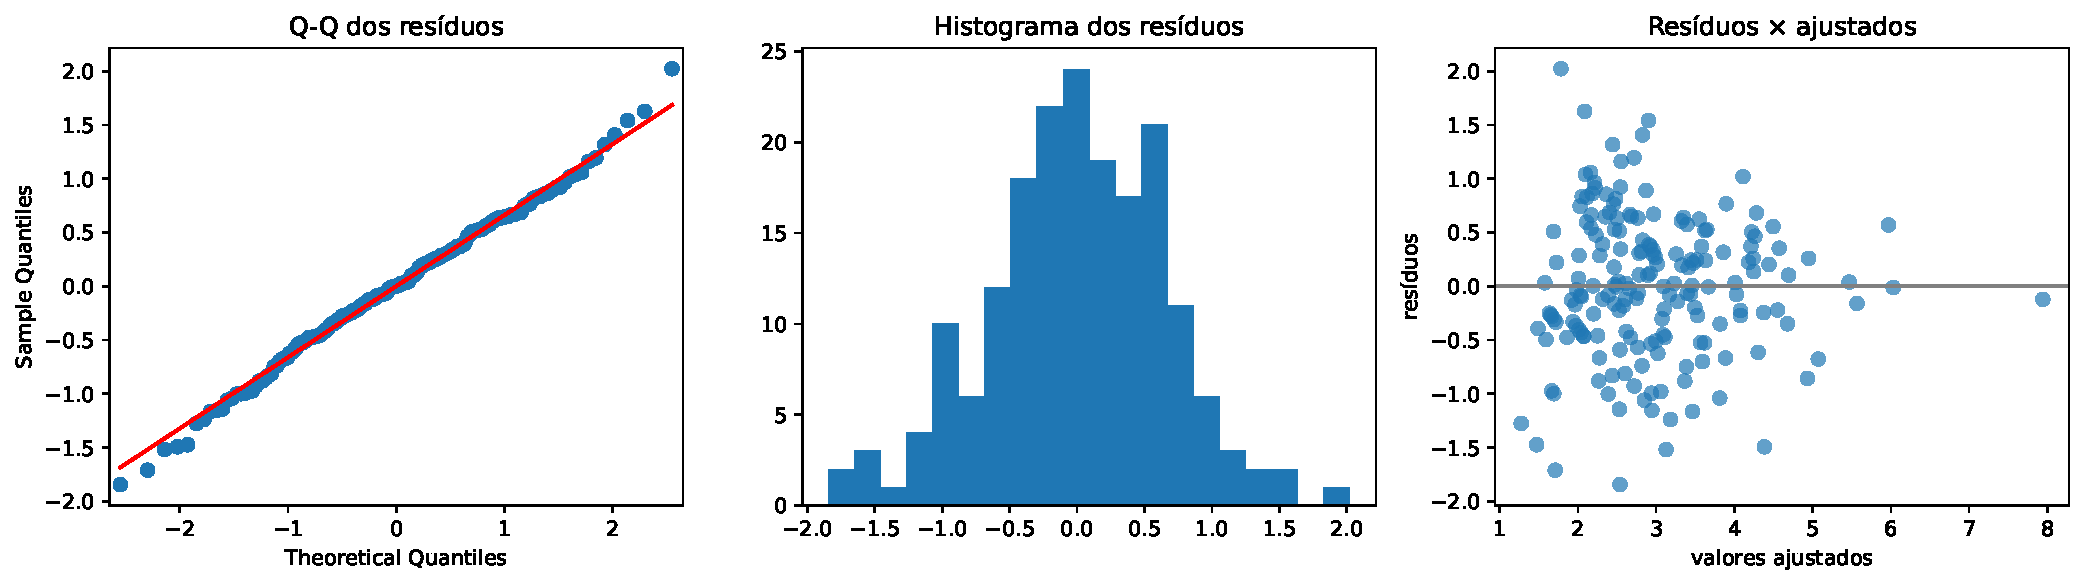
\includegraphics[width=\textwidth]{figuras/residuos_multiplo.pdf}
	\end{figure}
	\fonte{\fontedados}
	
	\begin{table}[H]
		\centering
		\caption{Testes de diagnóstico do modelo de regressão múltipla}
		\label{tab:diagnostico}
		\resizebox{\textwidth}{!}{%
			\begin{tabular}{llcl}
				\toprule
				\textbf{Pressuposto} & \textbf{Teste} & \textbf{Resultado} & \textbf{Conclusão (5\%)} \\
				\midrule
				Normalidade dos resíduos & Shapiro-Wilk  & $W = 0{,}996$; $p = 0{,}916$ & não se rejeita a normalidade \\
				Homocedasticidade        & Breusch-Pagan & $p = 0{,}036$                & heterocedasticidade leve \\
				Multicolinearidade       & VIF           & 1,355                        & ausente \\
				Pontos influentes        & Cook (máximo) & 0,128                        & nenhum ponto domina o ajuste \\
				\bottomrule
		\end{tabular}}
	\end{table}
	\fonte{\fontedados}
	
	Observa-se, na Figura~\ref{fig:residuos}, que os pontos do gráfico Q-Q acompanham a reta de referência e que o histograma é aproximadamente simétrico e centrado em zero, resultado confirmado pelo teste de Shapiro-Wilk ($p = 0{,}916$) na Tabela~\ref{tab:diagnostico}. O pressuposto de normalidade, portanto, é atendido.
	
	No gráfico de resíduos contra valores ajustados, os resíduos se distribuem em torno de zero sem padrão curvo, o que sustenta a forma linear do modelo. A amplitude dos resíduos, contudo, é maior entre os valores ajustados baixos, que correspondem aos municípios pequenos. O teste de Breusch-Pagan ($p = 0{,}036$) confirma essa heterocedasticidade leve, que não enviesa os coeficientes, mas pode tornar os erros padrão menos precisos; dado que os $p$-valores dos dois coeficientes estão muito abaixo de 5\%, as conclusões sobre sua significância não dependem dessa imprecisão.
	
	As maiores distâncias de Cook ocorrem em São João do Jaguaribe (0,128), São Gonçalo do Amarante (0,119), Eusébio (0,058), Pereiro (0,045) e Antonina do Norte (0,037), todas muito abaixo de 1. São Gonçalo do Amarante e Eusébio têm PIB per capita muito acima da média estadual, e Antonina do Norte é um dos municípios sem nenhum caso no período, o que explica por que se destacam; nenhum deles, porém, altera de forma relevante a reta estimada.
	
	O caso de São João do Jaguaribe merece destaque. O município registrou 44 CVLI no triênio com apenas 5.855 habitantes, o que equivale a cerca de 250 mortes por 100 mil habitantes por ano, mais de sete vezes a média estadual do período (35 por 100 mil). Esse desvio tem explicação conhecida: o município chegou a liderar a taxa de homicídios do país (DIÁRIO DO NORDESTE, 2022), com taxa de 224 por 100 mil entre 2019 e 2021 (O POVO, 2022b), e fica no Vale do Jaguaribe, a região do interior com a maior taxa de homicídios entre 2009 e 2023, onde o rompimento de um grupo criminoso com a facção Guardiões do Estado foi apontado pela Polícia Civil como causa de parte das mortes (O POVO, 2024b). Fatores locais desse tipo não são captados pela população nem pelo PIB per capita e aparecem no modelo como resíduos grandes.
	
	\subsection{Previsões}
	
	\begin{table}[H]
		\centering
		\caption{Previsão do número de CVLI (2021--2023) para um município com 100.000 habitantes e PIB per capita mediano}
		\label{tab:previsao}
		\begin{tabular}{lcc}
			\toprule
			\textbf{Medida} & \textbf{Escala do modelo} & \textbf{Número de casos} \\
			\midrule
			Valor previsto                                 & 4,286            & 71,7 \\
			Intervalo de confiança de 95\% (média)         & [4,065; 4,507]   & [57,3; 89,7] \\
			Intervalo de previsão de 95\% (um município)   & [2,952; 5,620]   & [18,2; 274,8] \\
			\bottomrule
		\end{tabular}
	\end{table}
	\fonte{\fontedados{} PIB per capita mediano dos 184 municípios: R\$ 13.087,72.}
	
	Conclui-se, pela Tabela~\ref{tab:previsao}, que um município cearense com 100.000 habitantes e PIB per capita mediano (R\$ 13.087,72) tem, segundo o modelo, cerca de 72 CVLI esperados no triênio 2021--2023, o equivalente a aproximadamente 24 por ano. Os valores em número de casos foram obtidos revertendo a transformação ($e^{\hat{y}} - 1$).
	
	O intervalo de confiança indica que a média de municípios com esse perfil deve estar entre 57 e 90 casos. O intervalo de previsão para um município específico é muito mais largo, de 18 a 275 casos: o erro padrão dos resíduos de 0,667 na escala logarítmica corresponde a variações de cerca de 3,7 vezes para mais ou para menos na escala de casos. O modelo, portanto, é adequado para descrever o padrão médio dos municípios, mas tem precisão limitada para prever o valor de um município isolado, o que reforça a importância dos fatores locais não incluídos. Os casos de São João do Jaguaribe e de Itapipoca ilustram essa limitação: um conflito entre facções pode multiplicar os homicídios de um município em poucos meses, independentemente de seu porte ou de sua economia. Pelo mesmo motivo, em 2024 a maior taxa de homicídios por 100 mil habitantes do estado foi a de um município pequeno, Groaíras, enquanto os maiores números absolutos ficaram com Sobral, Juazeiro do Norte e Itapipoca (O POVO, 2025).
	
	\newpage
	
	\section{Conclusão}
	
	O estudo atingiu o objetivo de estimar e validar um modelo de regressão linear para o número de CVLI dos 184 municípios do Ceará no período de 2021 a 2023.
	
	Quanto à relação entre as variáveis, a população residente mostrou-se o principal fator associado ao número de CVLI ($r = 0{,}815$ em escala logarítmica), explicando sozinha 66,5\% da variabilidade entre os municípios. O PIB per capita apresentou associação positiva e moderada ($r = 0{,}560$) e, incluído no modelo múltiplo, elevou o coeficiente de determinação para 69,2\%, com contribuição significativa confirmada pelo teste $F$ entre modelos aninhados ($F = 16{,}20$; $p = 0{,}0001$).
	
	O modelo final,
	\[
	\widehat{\ln(\text{CVLI}+1)} = -12{,}591 + 0{,}967\,\ln(\text{população}) + 0{,}605\,\ln(\text{PIB per capita}),
	\]
	indica que, para municípios de mesmo nível econômico, os casos crescem aproximadamente na mesma proporção da população, e que, para municípios de mesmo porte, um PIB per capita maior se associa a mais CVLI. Esse segundo resultado reflete a concentração da violência letal em municípios urbanizados e economicamente dinâmicos, sobretudo na Região Metropolitana de Fortaleza, e não uma relação causal entre renda e violência. A elasticidade próxima de 1 também é coerente com a desconcentração da violência: a participação de Fortaleza nos CVLI caiu de 41,8\% (2009--2017) para 26,9\% (2021--2023), praticamente igual à sua fatia da população.
	
	Na validação, o modelo mostrou-se globalmente significativo ($F = 203{,}57$; $p < 0{,}001$), com resíduos compatíveis com a normalidade, ausência de multicolinearidade e nenhum ponto excessivamente influente. Um dos principais aprendizados foi a comparação entre escalas: o modelo na escala original alcança $R^2$ de 0,970, mas é dominado por Fortaleza e viola os pressupostos, o que mostra que um $R^2$ alto não valida um modelo por si só.
	
	Como limitações, destacam-se a heterocedasticidade leve dos resíduos, que poderia ser tratada com erros padrão robustos; o uso de dados agregados por município, que não permite conclusões sobre indivíduos; o PIB per capita como indicador indireto de urbanização; e a ausência de variáveis sobre a atuação de grupos criminosos, desigualdade e estrutura etária. Os resíduos mais altos, como o de São João do Jaguaribe, correspondem justamente a municípios em que a imprensa registrou disputas entre facções, o que sugere que a presença e a dinâmica desses grupos é a principal variável omitida. Trabalhos futuros podem incluir essas variáveis e testar modelos próprios para dados de contagem, como a regressão de Poisson ou binomial negativa.
	
	\newpage
	
	\section{Referências Bibliográficas}
	
	\begin{description}
		\item BANCO DO NORDESTE. \textbf{Censo Demográfico 2022: primeiros resultados --- Ceará}. Fortaleza: BNB/Etene, 2023. Disponível em: \url{https://bnb.gov.br/s482-dspace/bitstream/123456789/1794/5/2023_CDPR_CE.pdf}. Acesso em: 26 out. 2026.
		
		\item BREUSCH, T. S.; PAGAN, A. R. A simple test for heteroscedasticity and random coefficient variation. \textbf{Econometrica}, v. 47, n. 5, p. 1287--1294, 1979.
		
		\item BUSSAB, W. O.; MORETTIN, P. A. \textbf{Estatística básica}. 9. ed. São Paulo: Saraiva, 2017.
		
		\item CEARÁ. Secretaria da Segurança Pública e Defesa Social. \textbf{Estatísticas: dados detalhados --- indicadores detalhados 2009 a 2025}. Fortaleza, 2026. Disponível em: \url{https://www.ce.gov.br/sspds/estatisticas/dados-detalhados/}. Acesso em: 07 set. 2026.
		
		\item COOK, R. D. Detection of influential observation in linear regression. \textbf{Technometrics}, v. 19, n. 1, p. 15--18, 1977.
		
		\item DIÁRIO DO NORDESTE. \textbf{Cidade do Vale do Jaguaribe lidera taxa de homicídios no Brasil; Ceará é o 4º estado mais violento}. Fortaleza, 2022. Disponível em: \url{https://diariodonordeste.verdesmares.com.br/seguranca/cidade-do-vale-do-jaguaribe-lidera-taxa-de-homicidios-no-brasil-ceara-e-o-4-estado-mais-violento-1.3249478}. Acesso em: 26 out. 2026.
		
		\item DIÁRIO DO NORDESTE. \textbf{Censo 2022: veja raio-x do que mudou na população do Ceará em 12 anos}. Fortaleza, 2023a. Disponível em: \url{https://diariodonordeste.verdesmares.com.br/ceara/censo-2022-veja-raio-x-do-que-mudou-na-populacao-do-ceara-em-12-anos-1.3387041}. Acesso em: 26 out. 2026.
		
		\item DIÁRIO DO NORDESTE. \textbf{A população da sua cidade cresceu ou diminuiu? Veja o número de moradores de cada município do Ceará}. Fortaleza, 2023b. Disponível em: \url{https://diariodonordeste.verdesmares.com.br/ceara/a-populacao-da-sua-cidade-cresceu-ou-diminuiu-veja-o-numero-de-moradores-de-cada-municipio-do-ceara-1.3386663}. Acesso em: 26 out. 2026.
		
		\item DIÁRIO DO NORDESTE. \textbf{Número de prisões de integrantes de facção na Região Metropolitana supera o de Fortaleza}. Fortaleza, 2026. Disponível em: \url{https://diariodonordeste.verdesmares.com.br/seguranca/numero-de-prisoes-de-integrantes-de-faccao-na-regiao-metropolitana-supera-o-de-fortaleza-1.3726183}. Acesso em: 26 out. 2026.
		
		\item ECONOMIC NEWS BRASIL. \textbf{Fortaleza detém maior fatia do PIB estadual e São Gonçalo tem maior PIB per capita}. 21 dez. 2022. Disponível em: \url{https://economicnewsbrasil.com.br/2022/12/21/fortaleza-detem-maior-fatia-do-pib-estadual/}. Acesso em: 26 out. 2026.
		
		\item GUJARATI, D. N.; PORTER, D. C. \textbf{Econometria básica}. 5. ed. Porto Alegre: AMGH, 2011.
		
		\item IBGE. \textbf{Censo Demográfico 2022}: população residente, área territorial e densidade demográfica (Tabela 4714). Rio de Janeiro: IBGE, 2023. Disponível em: \url{https://sidra.ibge.gov.br/tabela/4714}. Acesso em: \textit{<dd mmm.>} 2026.
		
		\item IBGE. \textbf{Produto Interno Bruto dos Municípios}: base de dados 2010--2023. Rio de Janeiro: IBGE, 2025. Disponível em: \url{https://www.ibge.gov.br/estatisticas/economicas/contas-nacionais/9088-produto-interno-bruto-dos-municipios.html}. Acesso em: \textit{<dd mmm.>} 2026.
		
		\item IPECE. \textbf{Painel de Indicadores Socioeconômicos 2023}. Fortaleza: Instituto de Pesquisa e Estratégia Econômica do Ceará, 2023. Disponível em: \url{https://www.ipece.ce.gov.br/wp-content/uploads/sites/45/2023/12/Painel_Indicadores_2023.pdf}. Acesso em: 26 out. 2026.
		
		\item IPECE. \textbf{PIB Municipal 2022--2023}. Fortaleza: Instituto de Pesquisa e Estratégia Econômica do Ceará, 2025. Disponível em: \url{https://www.ipece.ce.gov.br/wp-content/uploads/sites/45/2025/12/PIB_Municipal_2022_2023.pdf}. Acesso em: 26 out. 2026.
		
		\item MONTGOMERY, D. C.; PECK, E. A.; VINING, G. G. \textbf{Introduction to linear regression analysis}. 5. ed. Hoboken: Wiley, 2012.
		
		\item O POVO. \textbf{Assassinatos voltam a crescer no Ceará após dois meses de sequência positiva}. Fortaleza, 7 jun. 2022a. Disponível em: \url{https://mais.opovo.com.br/jornal/farol/2022/06/07/assassinatos-voltam-a-crescer-no-ceara-apos-dois-meses-de-sequencia-positiva.html}. Acesso em: 26 out. 2026.
		
		\item O POVO. \textbf{No município mais violento do país, só um homicídio gerou denúncia em 2021}. Fortaleza, 5 jul. 2022b. Disponível em: \url{https://mais.opovo.com.br/jornal/cidades/2022/07/05/no-municipio-mais-violento-do-pais-so-um-homicidio-gerou-denuncia-em-2021.html}. Acesso em: 26 out. 2026.
		
		\item O POVO. \textbf{Guerra entre facções faz homicídios em Itapipoca crescem dez vezes em 2023}. Fortaleza, 22 jul. 2023a. Disponível em: \url{https://mais.opovo.com.br/jornal/cidades/2023/07/22/guerra-entre-faccoes-faz-homicidios-em-itapipoca-crescem-dez-vezes-em-2023.html}. Acesso em: 26 out. 2026.
		
		\item O POVO. \textbf{Uma leitura do PIB dos municípios do Ceará}. Fortaleza, 21 dez. 2023b. Disponível em: \url{https://mais.opovo.com.br/colunistas/jocelio-leal/2023/12/21/uma-leitura-do-pib-dos-municipios-do-ceara.html}. Acesso em: 26 out. 2026.
		
		\item O POVO. \textbf{Comitê da Alece aponta interiorização da violência armada no Ceará}. Fortaleza, 13 mar. 2024a. Disponível em: \url{https://www.opovo.com.br/noticias/ceara/2024/03/13/comite-da-alece-aponta-interiorizacao-da-violencia-armada-no-ceara.html}. Acesso em: 26 out. 2026.
		
		\item O POVO. \textbf{Vale do Jaguaribe: do Novo Cangaço à guerra de facções}. Fortaleza, 29 mar. 2024b. Disponível em: \url{https://mais.opovo.com.br/jornal/reportagem/2024/03/29/vale-do-jaguaribe-do-novo-cangaco-a-guerra-de-faccoes.html}. Acesso em: 26 out. 2026.
		
		\item O POVO. \textbf{Ceará terminou 2024 com 3.272 homicídios; aumento é de 10,16\%}. Fortaleza, 11 jan. 2025. Disponível em: \url{https://mais.opovo.com.br/jornal/cidades/2025/01/11/ceara-terminou-2024-com-3-272-homicidios-aumento-e-de-1016.html}. Acesso em: 26 out. 2026.
		
		\item SEABOLD, S.; PERKTOLD, J. Statsmodels: econometric and statistical modeling with Python. In: PYTHON IN SCIENCE CONFERENCE, 9., 2010, Austin. \textbf{Proceedings} [...]. Austin: SciPy, 2010. p. 92--96.
		
		\item SHAPIRO, S. S.; WILK, M. B. An analysis of variance test for normality (complete samples). \textbf{Biometrika}, v. 52, n. 3/4, p. 591--611, 1965.
	\end{description}
	
	\newpage
	
	\section{Anexos}
	
	Os anexos reproduzem os scripts do repositório do projeto, incluídos diretamente dos arquivos \texttt{.py} para que o relatório mostre exatamente o código executado.
	
	\subsection*{Anexo A --- Preparação dos dados do IBGE (\texttt{preparar\_ibge.py})}
	\addcontentsline{toc}{subsection}{Anexo A --- preparar\_ibge.py}
	\lstinputlisting[style=python]{preparar_ibge.py}
	
	\newpage
	\subsection*{Anexo B --- Análise de regressão (\texttt{analise\_regressao.py})}
	\addcontentsline{toc}{subsection}{Anexo B --- analise\_regressao.py}
	\lstinputlisting[style=python]{analise_regressao.py}
	
\end{document}